\subsection{Perception}
The perception module linearizes the laser scan.
The laser scan is a 2-dimensional point cloud,
in the form of an array of distances measured at increasing angles.
We linearize this point cloud with a one-pass algorithm that ensures that
the interpolation error is bounded by a given value.
This gives us a sequence of line segments that represents the perceived obstacles around the car.
These line segments are the input to the Planner.

\begin{figure}
\centering
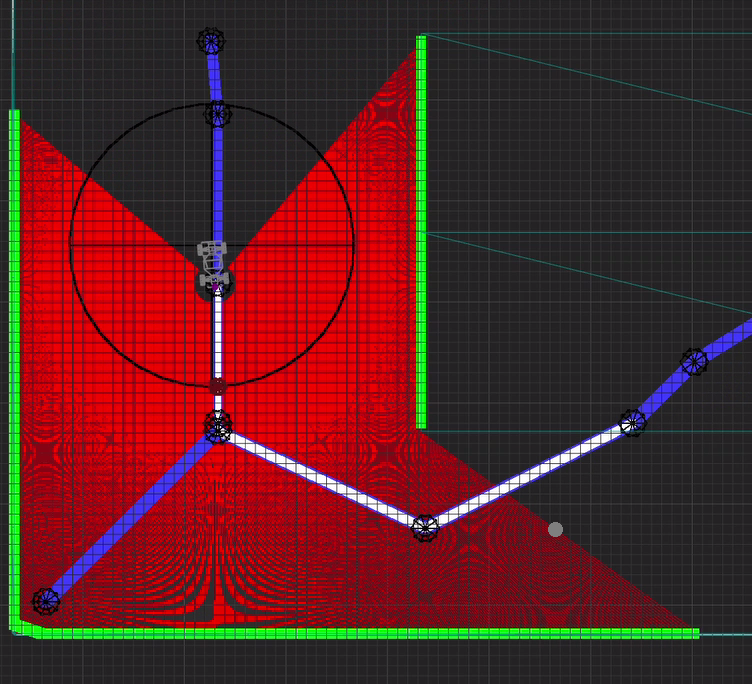
\includegraphics[width=88mm]{Figures/Planning.png}%
\label{fig:plan}%
\caption{The area visible by the laser scan is colored as red,
the linearized laser scan is in green,
the roadmap is in blue,
and the plan is in white.
The Pure Pursuit goal is a red dot on the lookahead circle.
The midpoint of the discontinuity of the (linearized) laser scan is a gray point.}
\end{figure}

